\documentclass[useAMS,usenatbib]{mn2e}
\usepackage[utf8]{inputenc}
\usepackage{graphicx}
\usepackage{amsmath}
\usepackage{amssymb}
%\usepackage[font={it},labelfont={bf}]{caption}
%\usepackage{units}
\usepackage{times}
\usepackage{color}
\usepackage[usenames,dvipsnames,svgnames,table]{xcolor}
\usepackage{xspace}
\usepackage{subcaption}

\usepackage{fixltx2e} % fixes placing of image positions

\definecolor{customhdrcolor}{rgb}{0.0,0.0,0.0}
\definecolor{customcitecolor}{rgb}{0.0,0.5,0.75}
\definecolor{customlinkcolor}{rgb}{0.0,0.5,0.75}

\usepackage[colorlinks=true,linkcolor=customlinkcolor,urlcolor=customlinkcolor,citecolor=customcitecolor,pdftex]{hyperref}

\ifpdf\pdfinfo{/Title      (Analysis of the Murchison radio environment for low-frequency astronomy)
               /Author     (A. R. Offringa et al.)
               /Keywords   (instrumentation: interferometers;methods: observational;techniques: interferometric;radio continuum: general)
        }
\else\usepackage{graphics}\fi

\setlength{\pdfpageheight}{\paperheight}
\setlength{\pdfpagewidth}{\paperwidth}

\newcommand{\editmark}[1]{#1}
%\newcommand{\editmark}[1]{{\color{red}{\textbf{#1}}}}

\newcommand{\degree}{\ensuremath{^{\circ}}\xspace}

% To make Dutch ``tussenvoegsels'' work correctly in Latex such as ``de Bruyn'', we use this command
% It fixes ordering and uppercases.
% In text, it should be written with uppercase, as in ``De Bruyn''
\DeclareRobustCommand{\TUSSEN}[3]{#2}

\title[The Murchison radio environment]{The low-frequency Murchison radio environment:\\interference analysis and mitigation}

\def\ANU{$^{1}$}
\def\CAASTRO{$^{2}$}
\def\Curtin{$^{3}$}

\author[A.~R.~Offringa et al.]{A.~R.~Offringa$^{1,2}$\thanks{\editmark{Corresponding author.} E-mail: \url{andre.offringa@anu.edu.au}},
R.~B.~Wayth\Curtin$^,$\CAASTRO,
N.~Hurley-Walker\Curtin,
D.~Kaplan\Curtin,
... , %\newauthor
builders list
\\
\ANU{}Research School of Astronomy and Astrophysics, Australian National University, Canberra, ACT 2611, Australia \\
\CAASTRO{}ARC Centre of Excellence for All-sky Astrophysics (CAASTRO), Australian National University, Canberra, ACT 2611, Australia \\
\Curtin{}International Centre for Radio Astronomy Research, Curtin University, Bentley, WA 6102, Australia\\
}

\begin{document}

\date{Accepted TODO. Received TODO; in original form TODO}
\pagerange{\pageref{firstpage}--\pageref{lastpage}}
\pubyear{2014}

\label{firstpage}
\maketitle

\begin{abstract}
...
\end{abstract}

\begin{keywords}
instrumentation: interferometers -- methods: observational -- techniques: interferometric -- radio continuum: general
\end{keywords}

\section{Introduction}
In recent years, the issue of radio-frequency interference (RFI) in radio astronomy caused by man-made transmitters has become larger due to an increased number of transmitters and wider frequency bandwidths of radio observatories. Spectrum allocation management and radio-quiet zones help to limit the interference, but do not solve interference from air-based transmitters or accidential electromagnetic radiation, for example from cars or wind turbines.

While some success has been seen in filtering interference from observations in which the data samples are cleaned from the contribution of interference \citep{spatial-filtering-parkes-multibeam-for-pulses,rfi-spatial-processing-hellbourg-2014}, such an approach is often not feasible due to technical limitations or the type of RFI. Therefore, a common approach is detection of contaminated data and ignoring these samples in further data analysis \citep{post-correlation-rfi-classification}. The consequence of the latter approach is that a certain amount of data is lost due to interference, and that frequencies that are continuously occupied by transmitters can not be observed. Analysing the results of interference detection and improving the understanding of RFI contamination can aid in several ways: understanding the effects on the science; improved observation scheduling; designing hardware and location of future telescopes with a maximal cost/benefit approach; and enforcing spectrum management strategies that are most beneficial for the observatories.

In this article, we will look specifically at the RFI situation of the MWA \citep{mwa}. The MWA is a low-frequency array consisting of 128 tiles, each with 16 dual-polarized dipoles, which allow observing between 80--300~MHz with a 31-MHz instantaneous bandwidth. Its main science driver is to detect redshifted 21-cm radio signals from the Epoch of Reionization (EoR; \citealt{bowman-science-with-the-mwa-2013}). To avoid as much RFI as possible, the MWA is located in the Murchison region in Western Australia. Analysing the interference situation of the MWA can improve the MWA observing and processing strategy, and will additionally also provide valuable information for the Square Kilometre Array (SKA), because the cores of the SKA low-frequency aperture arrays and SKA mid-frequency survey dishes are planned to be build near the location of the MWA.

The interferometric arrays LOFAR, PAPER and the Long Wavelength Array (LWA) are all designed to perform 21-cm EoR science, and all observe in approximately the same frequency range as the MWA. Comparing the MWA to these arrays therefore allows the comparison of the observatory site and hardware design with respect to the RFI mitigation effectivity. In \citet{lofar-radio-environment} it has been shown that the radio environment of LOFAR does not pose any issues on regular observations despite that, unlike the MWA, LOFAR is build in a populated area. This is confirmed by \citet{ncp-eor-yatawatta}, where the authors analyse the first imaging of EoR long-integration observations with LOFAR. They reach near-thermal noise sensitivity, and argue that RFI is not a limitation for further increasing the sensitivity. Further analysis showed that RFI models for LOFAR can estimate the leakage of the RFI detection \citep{offringa-rfi-distributions}. Those analyses concluded that with sufficient precautions, such as good receiver design and accurate detection methods, the leaked RFI is weak and averages down similar to Gaussian noise.

TODO paper structure.

\section{Method}
RFI detection, often referred to as ``data flagging'', is one of the first steps in the data processing. It is important to perform initial data flagging at high time and frequency resolution, because this increases detection accuracy and decreases the loss of data \citep{lofar-radio-environment}. Consequently, RFI detection has to work on large data volumes, and its computational cost is therefore a concern -- in particular for many-element arrays. In some projects, simple thresholding is used to mitigate the worst interference, which is computationally cheap but not very accurate. For example, a $3\sigma$ threshold is used for reducing PAPER data in \citet{parsons-paper-eorlimit-2014}. Several observatories or projects have designed pipelines that include more advanced RFI mitigation. Examples of such pipelines include \textsc{aoflagger} \citep{post-correlation-rfi-classification,scale-invariant-rank-operator}, originally designed for LOFAR; \textsc{flagcal} for preprocessing data from the Giant Metrewave Radio Telescope (GMRT; \citealt{prasad-flagcal-2012}); and \textsc{serpent} for preprocessing data from the Multi-Element Radio Linked Interferometer Network (e-MERLIN; \citealt{serpent-peck-2013}). For RFI detection in MWA observations, LOFAR's \textsc{aoflagger} is used. This flagger has shown to have a good accuracy, is fast and has a library interface, which allows it to be integrated in a pipeline.

\subsection{The AOFlagger}

\begin{figure}
\begin{center}\hspace*{-0.8cm}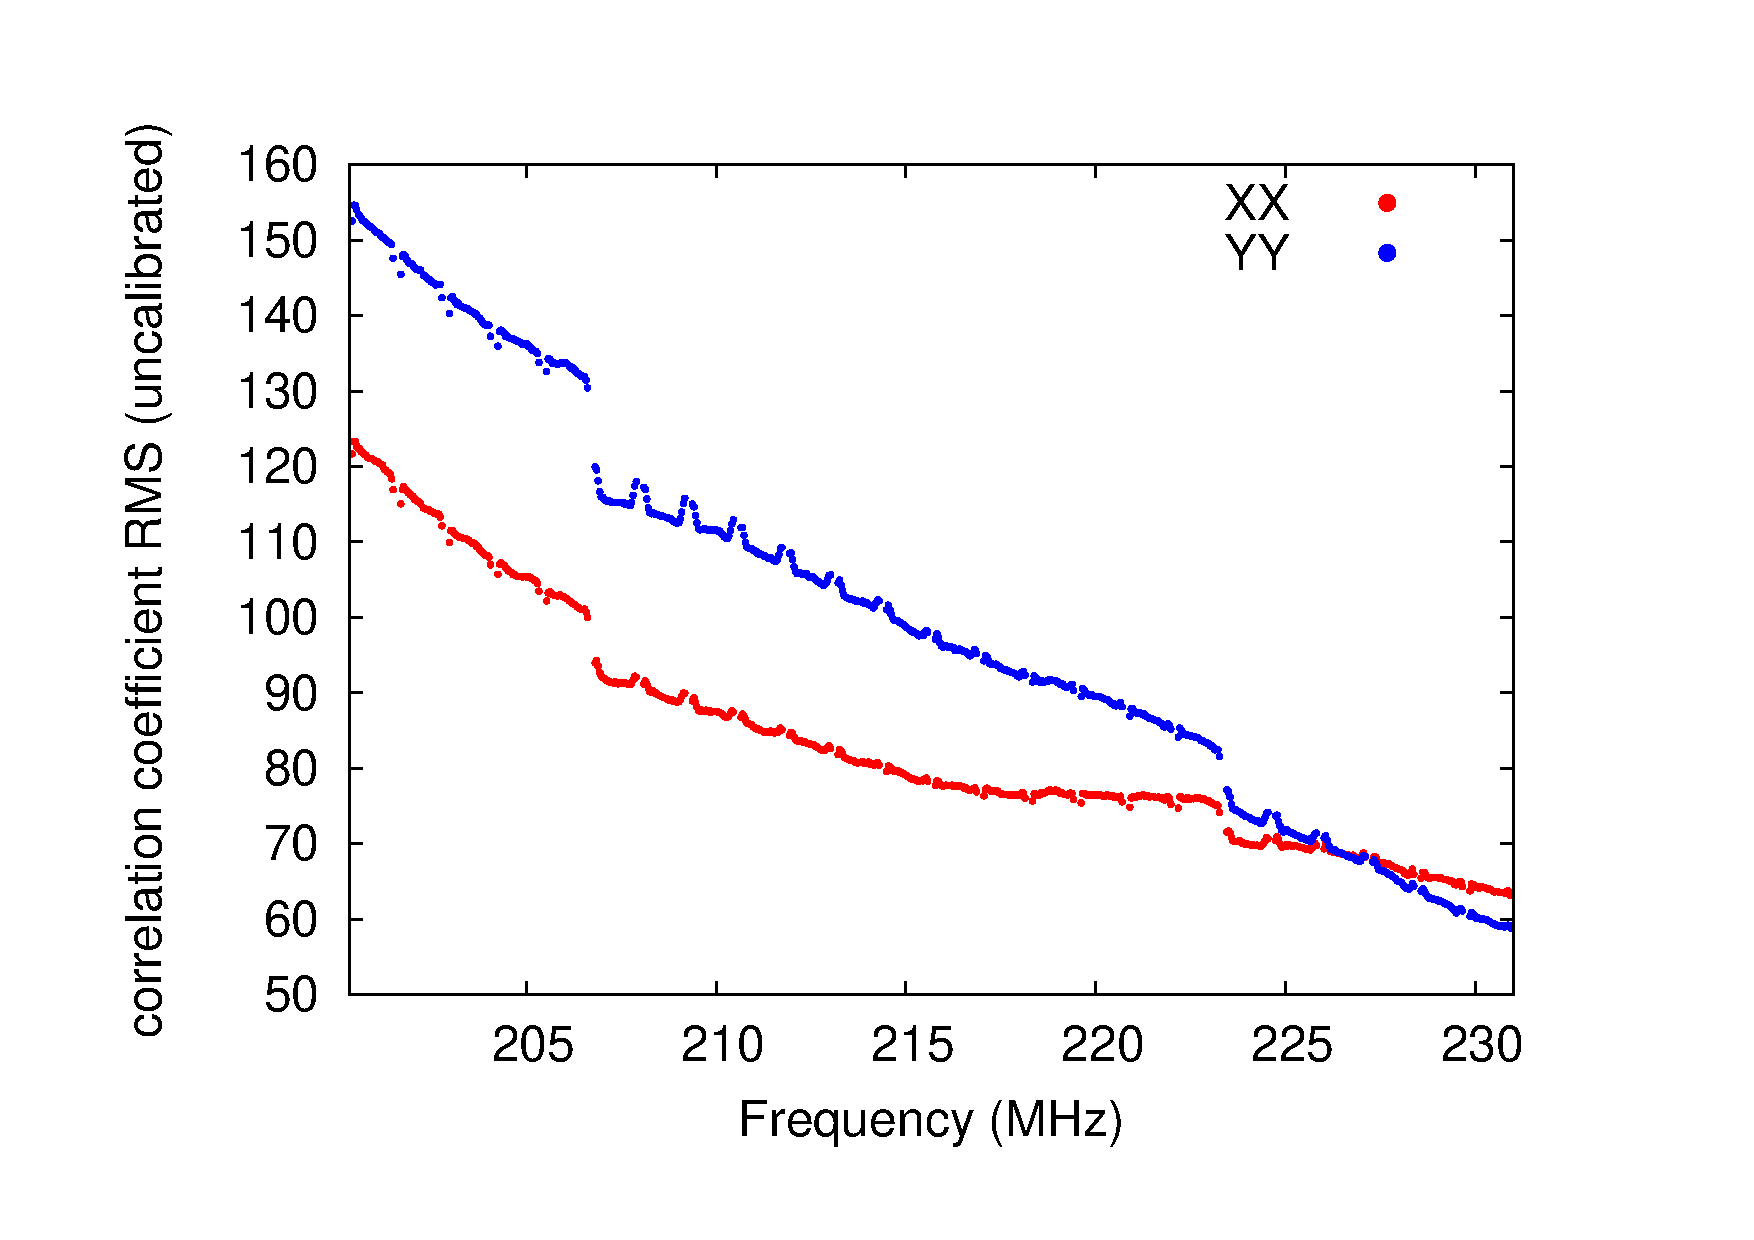
\includegraphics[width=10.5cm]{img/bandpass}
\caption{Correlator output RMS over frequency in an MWA high-frequency observation, calculated over all cross-correlated baselines and 112 seconds of data. In this band, the band-pass shows two large discontinuities over frequency, because the MWA receivers apply different digital gains at different frequencies to minimize quantization noise. TODO explain subband bandpass somewhere %TODO
}
\label{fig:bandpass}
\end{center}
\end{figure}

To detect RFI in MWA observations, we have used the \textsc{aoflagger} and implemented this as a standard MWA tool to flag all MWA data. The \textsc{aoflagger} allows customizing its flagging strategy, such as changing the threshold levels and expected smoothness of good data. Optimal values vary from telescope to telescope because of different band-pass shapes, different time and frequency resolutions and varying field of views. Specific strategies for several telescopes have been implemented in the \textsc{aoflagger} software, including an MWA specific strategy which is used in this work. The different \textsc{aoflagger} strategies are variations on the original LOFAR strategy described in \citet{lofar-radio-environment}. In the LOFAR strategy, the sky contribution is estimated by applying a 2-dimensional high-pass filter on the visibility amplitudes of each baseline in the time and frequency direction. Subsequently, line-shaped features are detected by the \textsc{sumthreshold} method, which is a combinatorial threshold method \citep{post-correlation-rfi-classification}. After iterating these steps a few times, the scale-invariant rank (SIR) operator is applied on the two-dimensional flag mask. The SIR operator is a morphological technique to search for contaminated samples \citep{scale-invariant-rank-operator}.

The MWA and LOFAR strategies differ on one aspect. For the MWA, an extra bandpass correction is added, which is performed by dividing the bandwidth in 48 parts and dividing each part by its Winsorized standard deviation. This step is required to smooth out discontinuities due to varying digital gains over frequency that are applied by the receivers to minimize quantization noise. An example of these discontinuities is shown in Fig.~\ref{fig:bandpass}. The bandpass corrections are not permanently applied to the data, but only applied during flagging. Normally, a per-channel calibration is performed after flagging for getting accurate flux calibration, which corrects the gain discontinuities permanently. Recently, the applied digital gains have been smoothed to prevent these discontinuities, which makes it possible to skip the band-pass correction step, but this step was still included in this work. 

In this work, \textsc{aoflagger} version 2.6 released on 26 June 2014 is used.

\subsection{\textsc{cotter}: the MWA preprocessing pipeline}

The \textsc{aoflagger} software provides a C++ library\footnote{\url{http://aoflagger.sourceforge.net/doc/api/}} that can be integrated in a pipeline, thereby minimizing reading/writing of data. We have written an MWA-specific preprocessing pipeline named \textsc{cotter} that uses the \textsc{aoflagger} library for RFI detection. Additionally, \textsc{cotter} performs the following steps: it converts the raw correlator files into \textsc{casa} measurement sets or uvfits files; applies bandpass gain corrections; corrects the phases for varying cable lengths; calculates the $uvw$-coordinates; applies phase tracking to the desired sky coordinates; flags samples from the correlator that are missing or incorrect; and allows averaging the observation in frequency or time direction to reduce the data volume. It also collects various statistics and writes these into a measurement set using the LOFAR quality statistics format\footnote{Described in ``MeasurementSet description for LOFAR version 2.08'' by Schoenmakers \& Renting.}. Various tools are available to analyse these statistics, e.g. the \textsc{aoqplot} tool that is part of the \textsc{aoflagger} software can plot the statistics over various dimensions in an interactive manner.

MWA observations are split into snapshots of a few minutes by the correlator. The MWA archive stores the raw correlator outputs for every snapshot as an observation that can be referenced by its observation ID. For more details about the correlator, see TODO fix reference Ord et al. (2014). Currently, the \textsc{cotter} preprocessing pipeline is ran by the scientist that calibrates and images the data. Once the scientist has downloaded the raw files for a given observation ID, there are various ways of processing MWA data. For imaging MWA data with the Real-Time System (RTS; \citealt{rts-mwa-2008}), \textsc{cotter} is ran in a special mode such that it only flags the data, and does not convert the raw correlator files. After running \textsc{cotter}, the raw files and a flag mask are given as input to the RTS. For more traditional data processing with e.g. \textsc{casa} or \textsc{miriad}, the \textsc{cotter} output is set to either the \textsc{casa} or uvfits format. The output is then directly readable by the astronomical software.

One particular issue in implementing \textsc{cotter} is that both the raw correlator files and the desired output files are ordered in time, but flagging is done baseline by baseline. The \textsc{sumthreshold} technique and the scale-invariant rank operator that are used by the flagging strategy, use statistics over large time and frequency ranges. Therefore, accuracy is improved when the time-frequency flagging intervals are as large as possible. However, a typical snapshot is about 50 GB in size, and without increasing reading and writing, it requires thus 50 GB of memory to perform flagging on the full data. When less memory is available, \textsc{cotter} will split the observation in different time chunks and flags those independently. The \textsc{ndppp} software used by LOFAR (TODO reference?) uses a similar partitioning of data to overcome the time-ordering problem. Partitioning the data has the undesirable behaviour that executing \textsc{cotter} on a low-memory machine decreases its flagging accuracy. Because not all astronomers might have easily access to high-memory machines, a platform with sufficient memory has been setup that pre-runs \textsc{cotter} on all observations.

When time or frequency averaging is requested, \textsc{cotter} averages samples together that have not been flagged. When all input samples are flagged, the average of all input visibilities is stored into the the output sample, and the output sample is flagged. This method makes it possible to superficially analyse flagged samples in the output, even though information is lost in the averaging. \textsc{cotter} stores a weight for each visibility in the output file, which is scaled to the number of unflagged input samples that were used for the output sample. Because of this, when no averaging is requested, the output is 50\% larger than the input (one extra float per complex float visibility). In practice, most observations are recorded at a resolution of 0.5 s and 40 kHz, and averaged to a resolution of 2--4 s and 40--80 kHz to reduce the data volume. This does not significantly cause any time or bandwidth decorrelation up to the first beam nul. \textsc{cotter} performs the phase shifting and cable delay corrections before averaging, and recalculates the $uvw$ values for the central time and frequency of the output sample. This helps to prevent time/frequency decorrelation.

\section{Data description}

\begin{table*}
\caption{List of observations used in the analyses. The RFI column contains the fraction of visibilities that the initial \textsc{aoflagger} run has classified as RFI (which includes false positives). The DVB column displays the fraction of visibilities that were unusable because of the presence of DVB signals, and which the flagger does not flag. Because the DVB frequencies are only observed in GLEAM observations, this fraction is only given for those. }\label{tbl:obs-list}
\begin{tabular}{|l|l|r|r|r|c|}
\hline
\textbf{Project} &\textbf{Date} & \textbf{Frequencies (MHz)} & \textbf{Duration} & RFI & DVB \\
\hline
EoR high& 2013-08-23 & 167.0--197.7              & 3h & 0.53\% & ---\\
GLEAM & 2013-08-25 & 72.3--133.8, 138.9--230.8 & 7h & 0.94\% & 0\% \\
EoR low& 2013-08-26 & 138.9--169.6              & 6h & 0.81\% & ---\\
GLEAM & 2013-11-05 & 72.3--133.8, 138.9--230.8 & 7h & 1.27\% & 0\% \\
GLEAM & 2013-11-25 & 72.3--133.8, 138.9--230.8 & 7h & 0.69\% & 0\% \\
EoR high& 2014-02-05 & 167.0--197.7              & 6h & 0.54\% & -- \\
GLEAM & 2014-03-16 & 72.3--133.8, 138.9--230.8 & 7h & 0.79\% & 0\% \\
GLEAM & 2014-03-17 & 72.3--133.8, 138.9--230.8 & 7h & 1.64\% & 3\% \\
EoR high& 2014-04-10 & 167.0--197.7              & 6h & 0.68\% & ---\\
GLEAM & 2014-06-18 & 72.3--133.8, 138.9--230.8 & 7h & 0.98\% & 0\% \\
RFI test&2014-08-27& 131.2--161.9     & 2$\times$8 m& 1.85\% & --- \\
\hline
\multicolumn{3}{|r|}{\textbf{Total}} & \textbf{63h} & \textbf{...\%} & \textbf{0.5\%}\\
\hline
\end{tabular}
\end{table*}

We analyze the RFI in 10 nights of data from two different MWA projects: the MWA EoR project \citep{bowman-science-with-the-mwa-2013} and the GaLactic and ExtrAgalactic MWA (GLEAM) survey (TODO cite Randall). The observations are listen in Table~\ref{tbl:obs-list}.

The MWA EoR project observes primarily in the 138.9--197.7~MHz range, covering the HI 21-cm line with redshift 6.1--9.2. Because the MWA has a 30.72~MHz instantaneous bandwidth, this range has been split up so that each night observes with a central frequency of either 154.2 or 182.4~MHz, with an overlap of 2.6 MHz. In these observations, the selected EoR field is tracked by the primary beam, such that the sensitivity towards the field is maximal.

The GLEAM survey covers 72.3--230.8 MHz split into 5 bands of 30.72 MHz. The GLEAM observations are made in drift-scan mode, and the 5 bands are observed one by one in 5 subsequent snapshots.

Both projects avoid the subbands that cover the frequency range 133.8--138.9~MHz, because the ORBCOMM low Earth orbitting (LEO) satellites transmit in these subbands. When these frequencies are observed, the subbands are often so strongly contaminated that it affects imaging sensitivity. For completeness, we include a 16-min observation that covers this frequency range.

\section{Detection results}

\noindent\begin{figure*}
\begin{center}\hspace*{-0.2cm}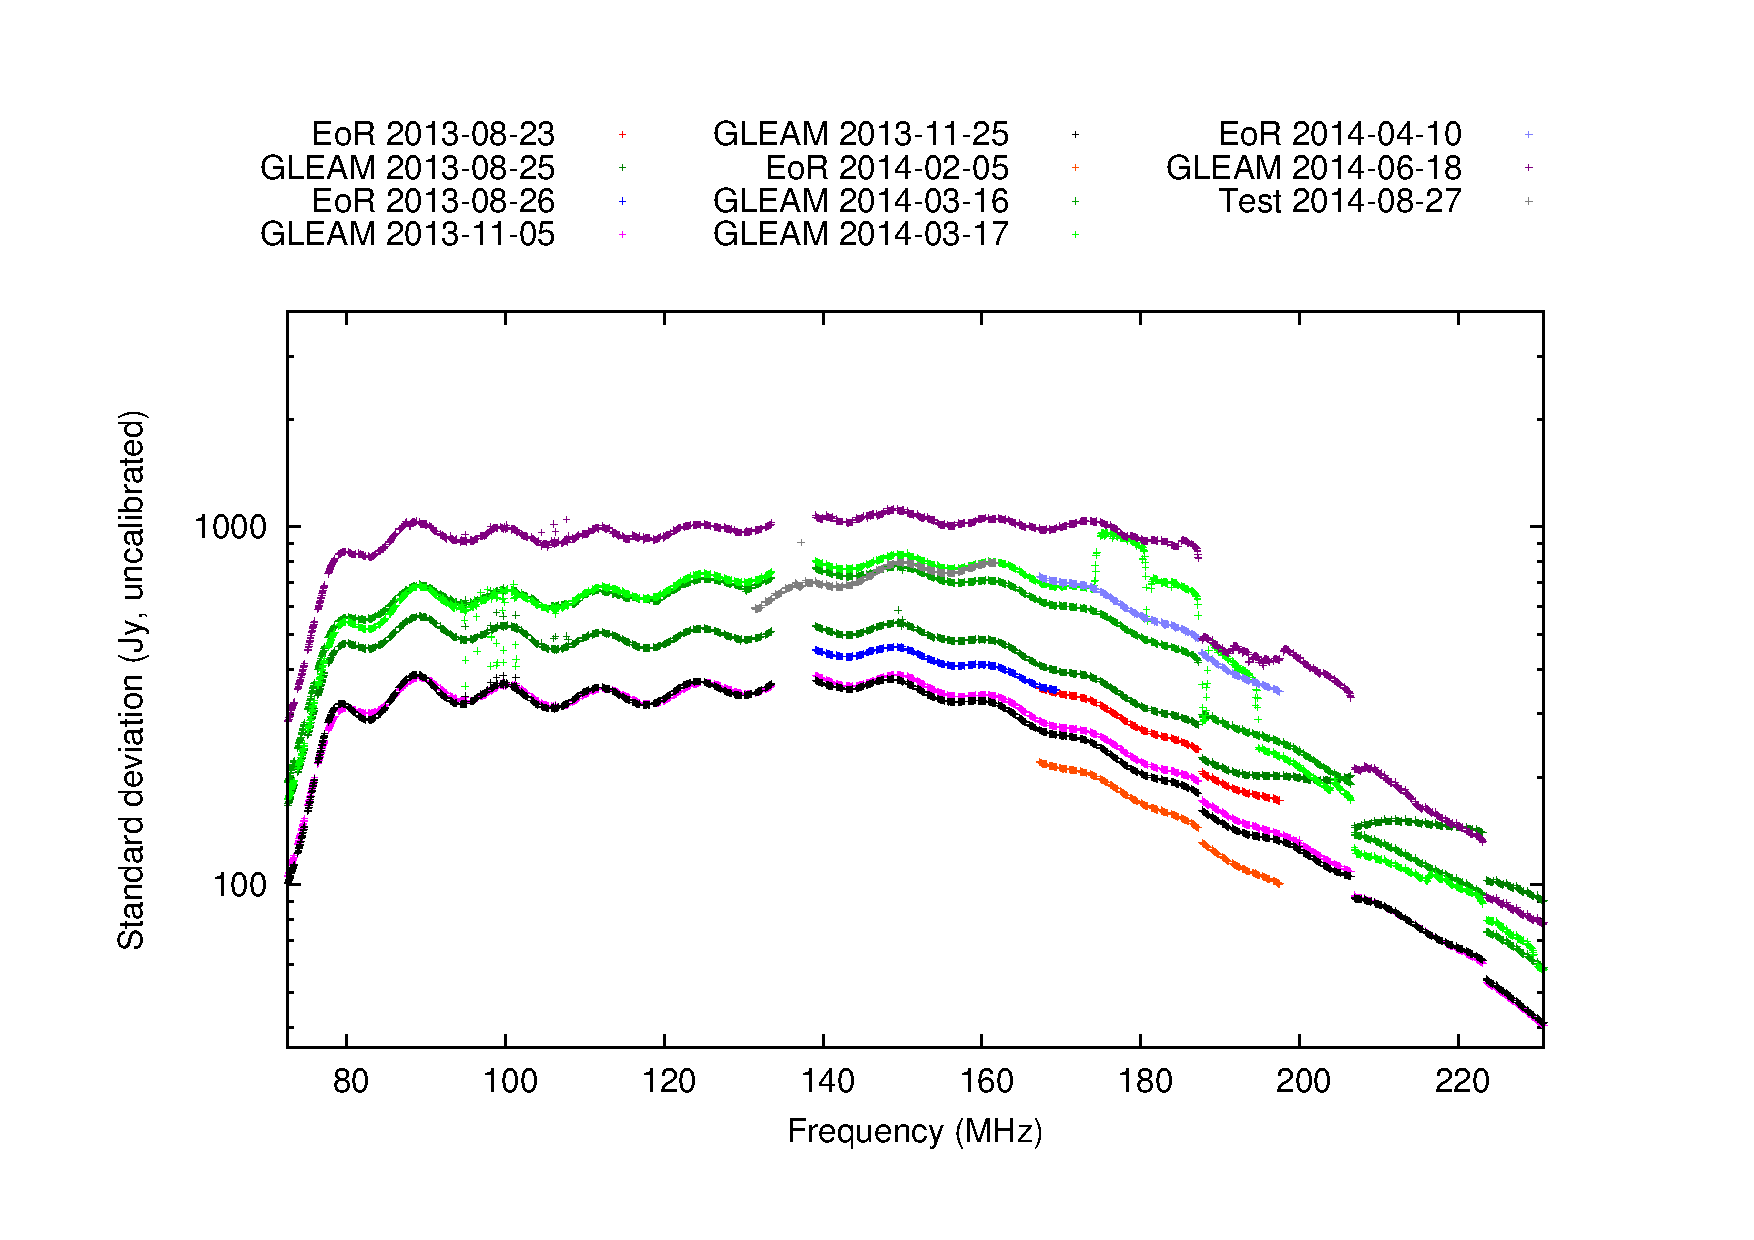
\includegraphics[width=18cm]{img/plot-stddev-per-set}\vspace{-1cm}
\caption{..}
\label{fig:stddev-per-set}
\end{center}
\end{figure*}


\noindent\begin{figure*}
\subcaptionbox{RFI contamination found in the 2 m amateur band (146 MHz).}[\linewidth]{%
% obs data: 1061583576, 2013-08-26.
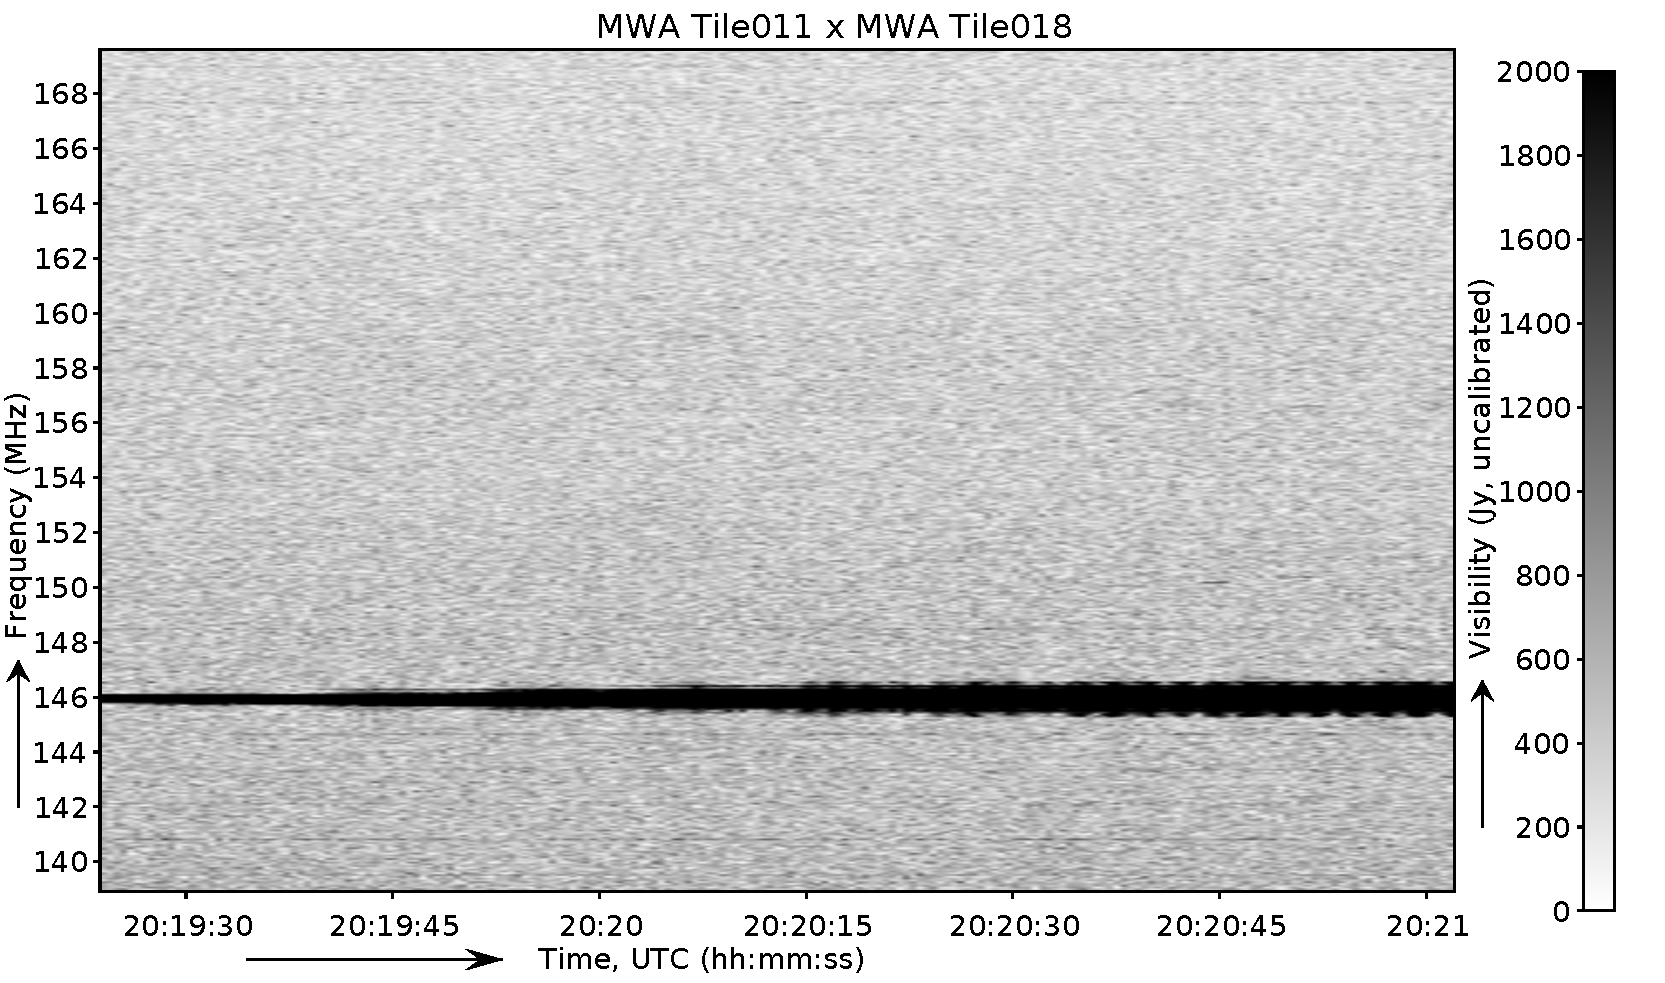
\includegraphics[width=9.1cm]{img/amateur-2m-band-example}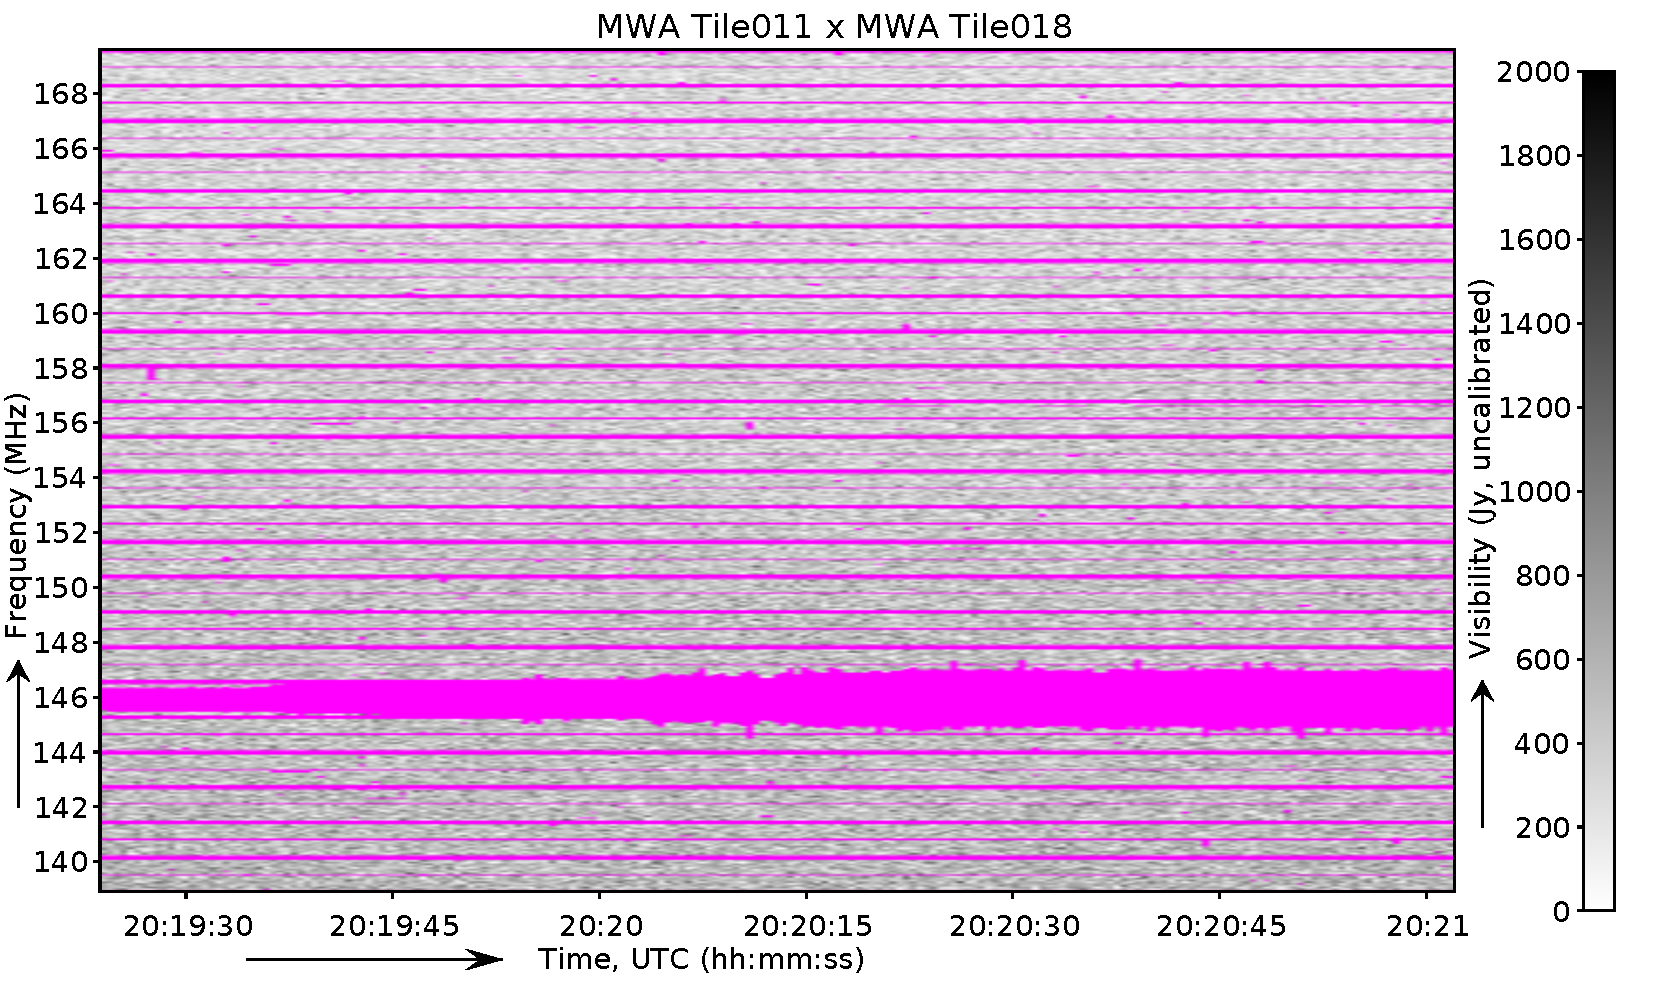
\includegraphics[width=9.1cm]{img/amateur-2m-band-flagged}
\label{fig:amateur-2m}
}\\\vspace{3mm}%
\subcaptionbox{Short RFI burst of 2 s centred on 150.17 MHz. This shows that flagging at high time and frequency resolution is necessary to accurately detect RFI.}[\linewidth]{%
% obs data: 1061583576, 2013-08-26.
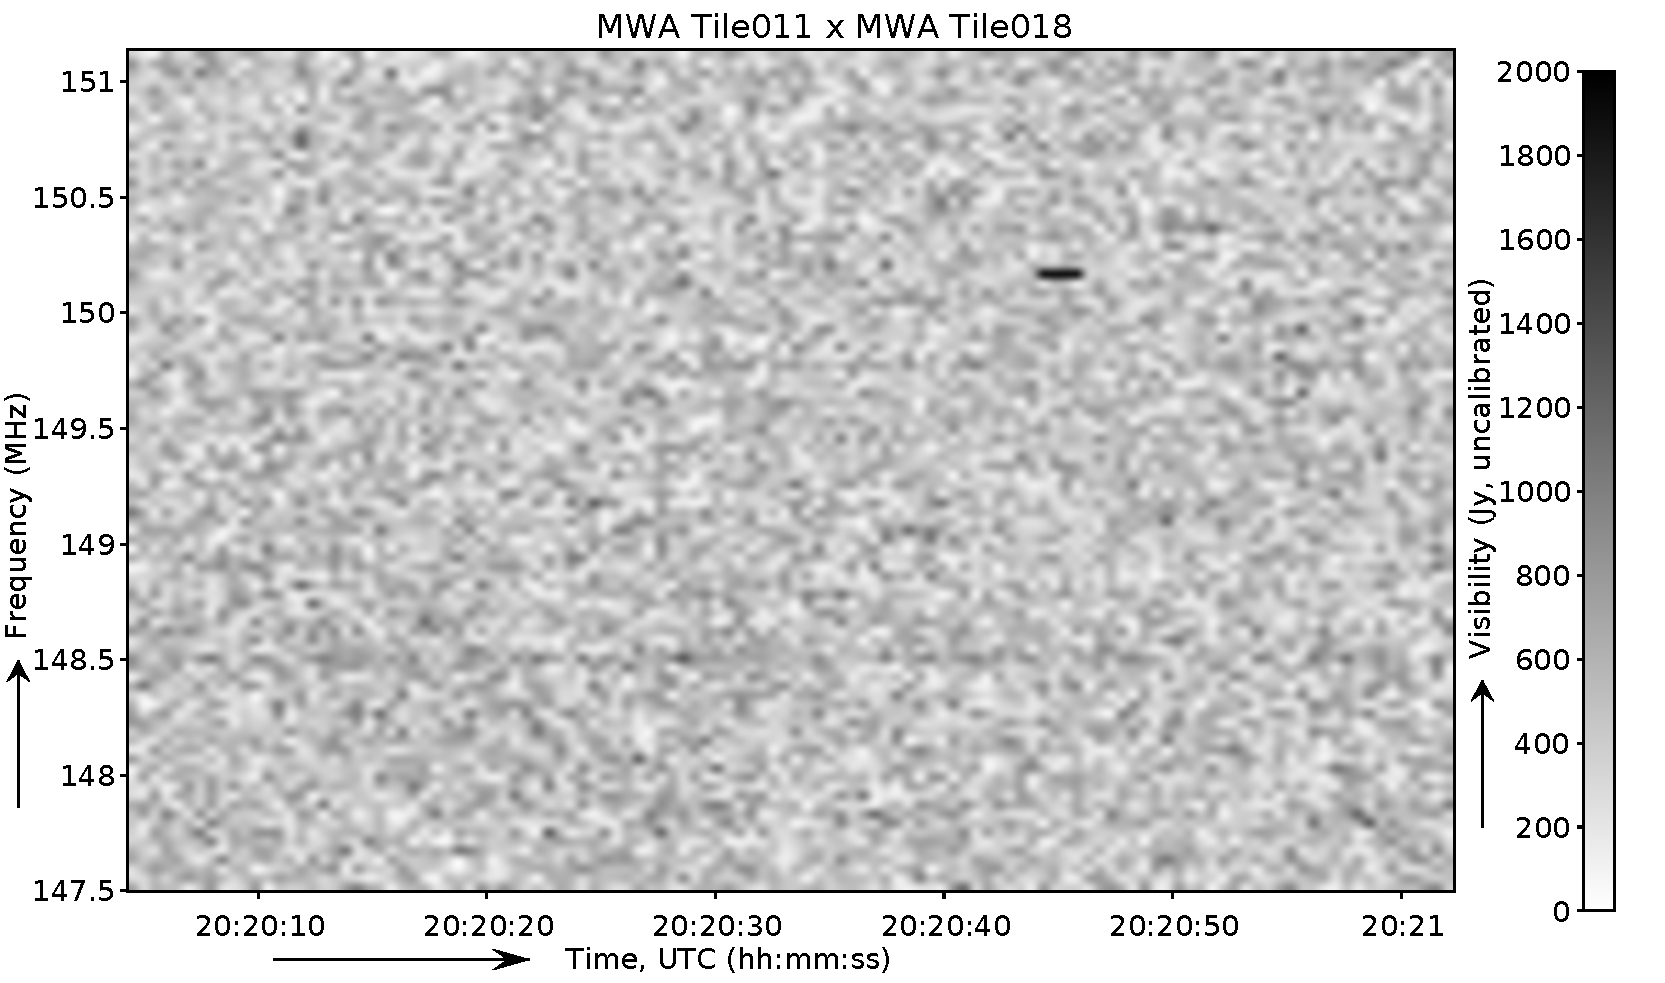
\includegraphics[width=9.1cm]{img/150_2_mhz_example}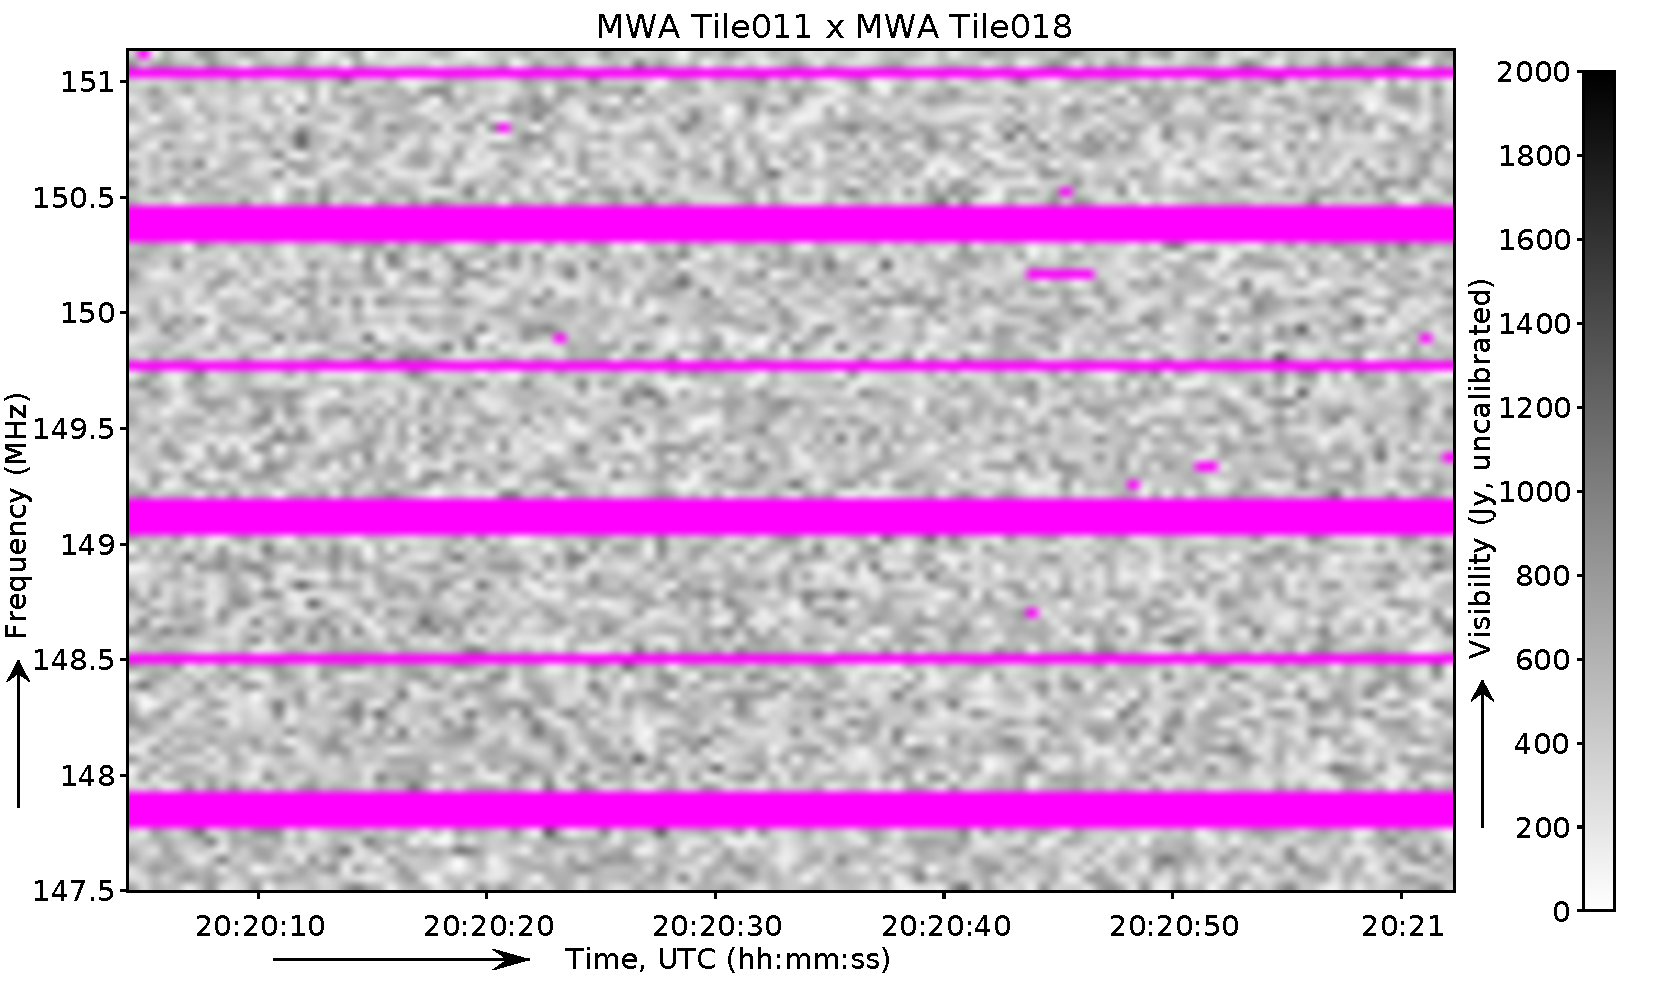
\includegraphics[width=9.1cm]{img/150_2_mhz_flagged}
\label{fig:150_2}
}\\\vspace{3mm}%
\subcaptionbox{A weakly-observed transmitter centred on 156.66 MHz. This same frequency is flagged in several correlations, and it can therefore be assumed this is real RFI. This is an example in which the AOFlagger detects an event that would not be detected by regular thresholding. }[\linewidth]{%
% obs data: 1061583576, 2013-08-26.
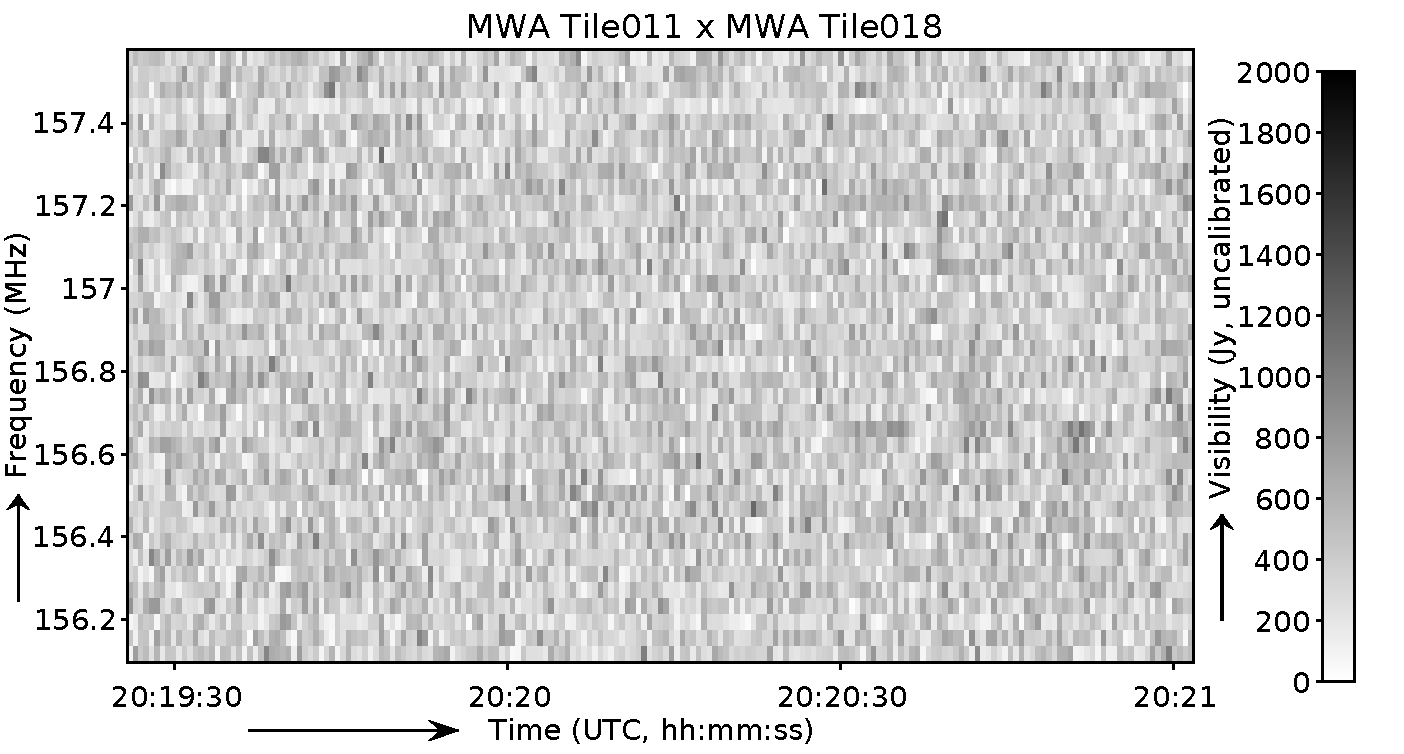
\includegraphics[width=9.1cm]{img/156_7_mhz_example}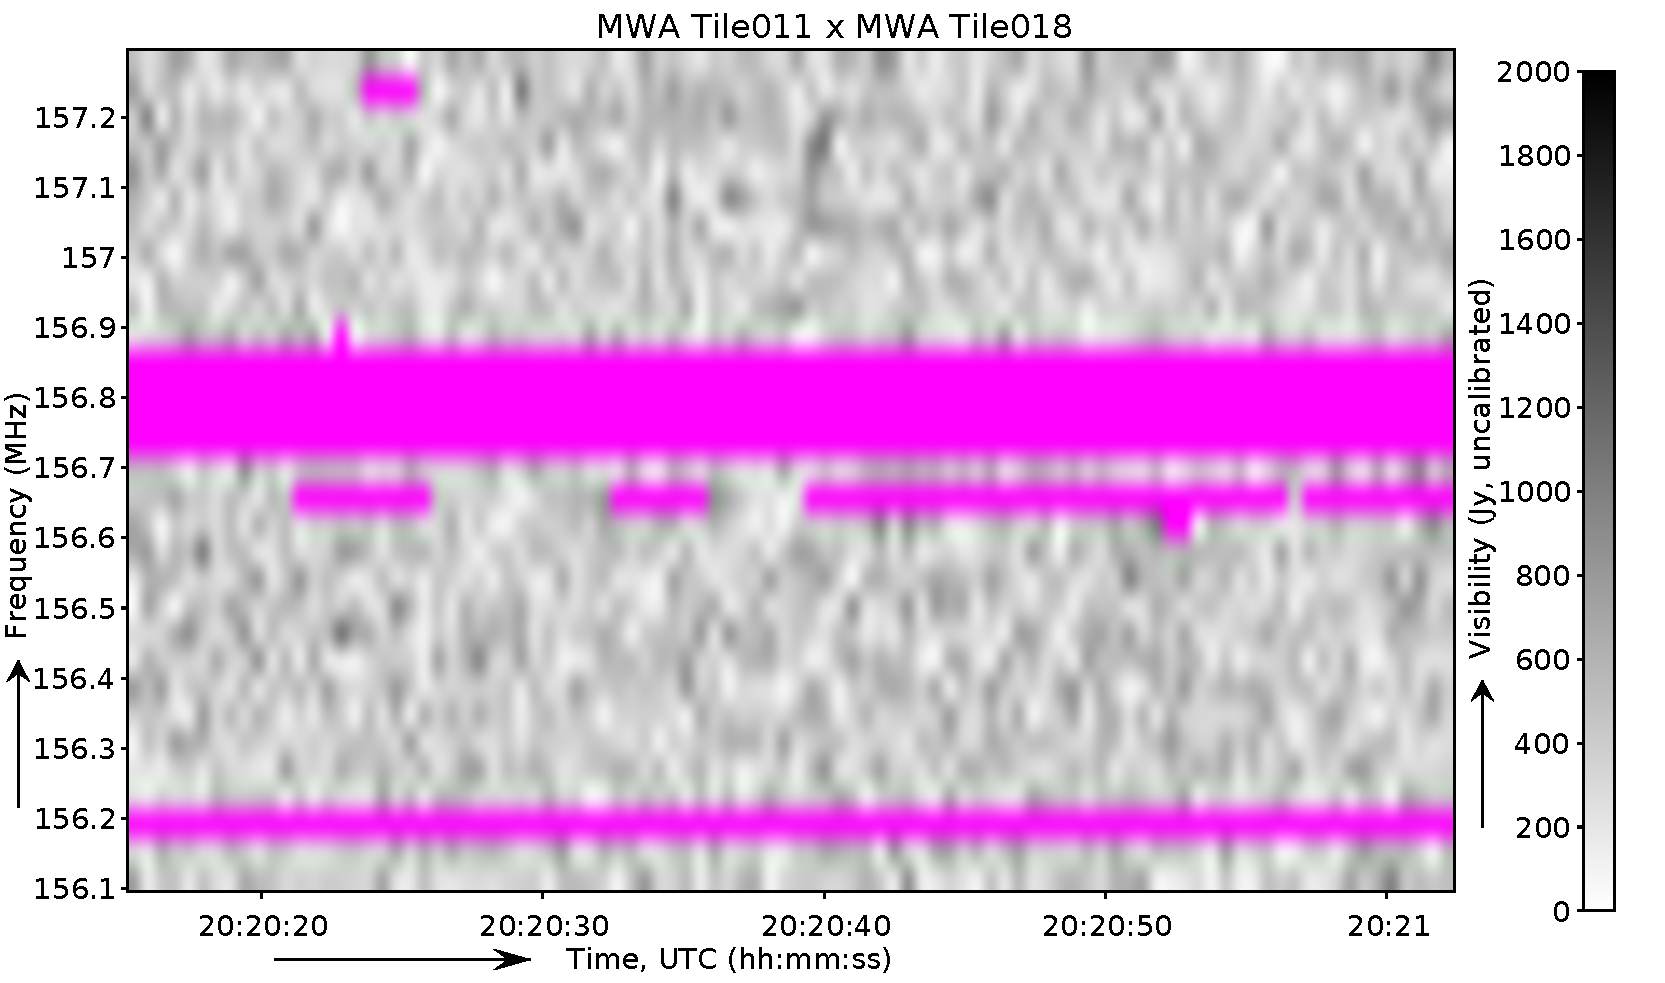
\includegraphics[width=9.1cm]{img/156_7_mhz_flagged}
\label{fig:156_7}
}%
\caption{Examples of RFI events found in the EoR low band (138.9--197.7 MHz) in a 2-min snapshot with relatively high RFI contamination. These panels show the Stokes I amplitudes. In the right figures, the result of RFI detection is shown with purple. The horizontally flagged lines are flagged because they are 1.28-MHz subband edge or centre channels, which are unusable because of aliasing of the poly-phase filter bank and DC offsets, respectively.}
\end{figure*}

\noindent\begin{figure}
% obs data: 1061583576, 2013-08-26.
\begin{center}\hspace*{-0.2cm}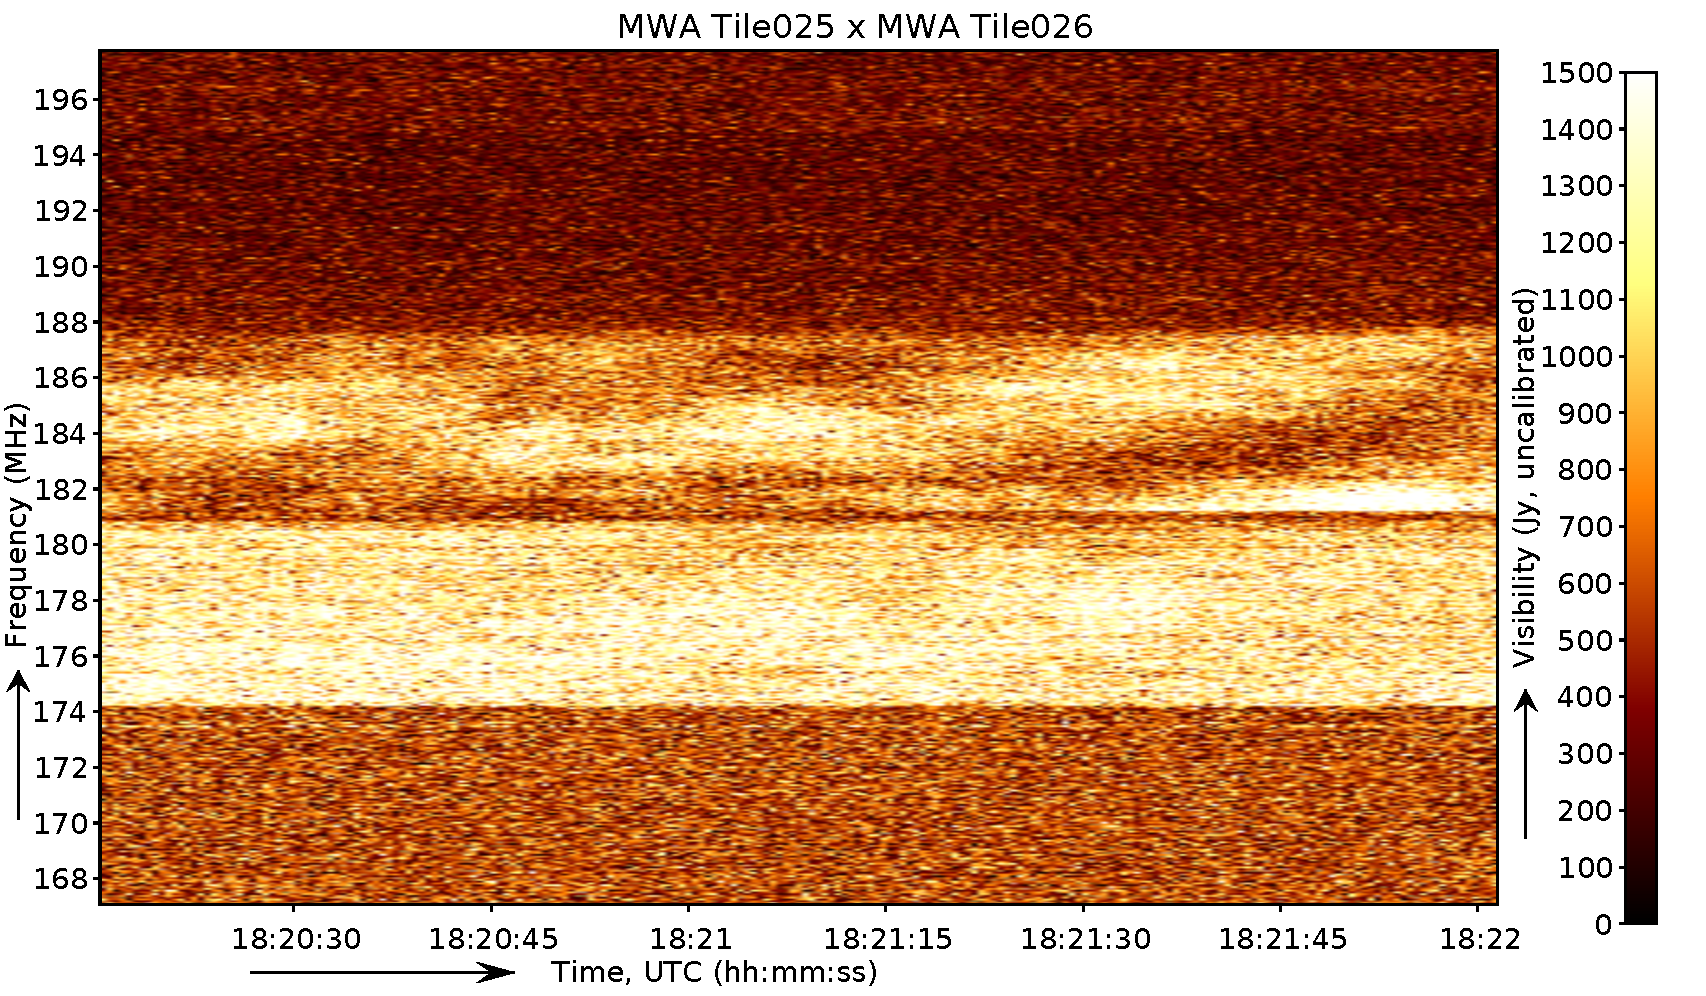
\includegraphics[width=9.1cm]{img/dvb_example}
\caption{RFI from Digital Video Broadcasting (DVB). Because of its broadband nature, this kind of RFI is not well flagged in the initial AOFlagger step, but is detectable in the global statistics. This type of RFI makes most of the 30.72~MHz bandwidth unusable. It is visible for about 2 h in 1 out of the 6 nights that observed this band. }
\label{fig:dvb_example}
\end{center}
\end{figure}

%\noindent\begin{figure*}
%\begin{center}\hspace*{-0.2cm}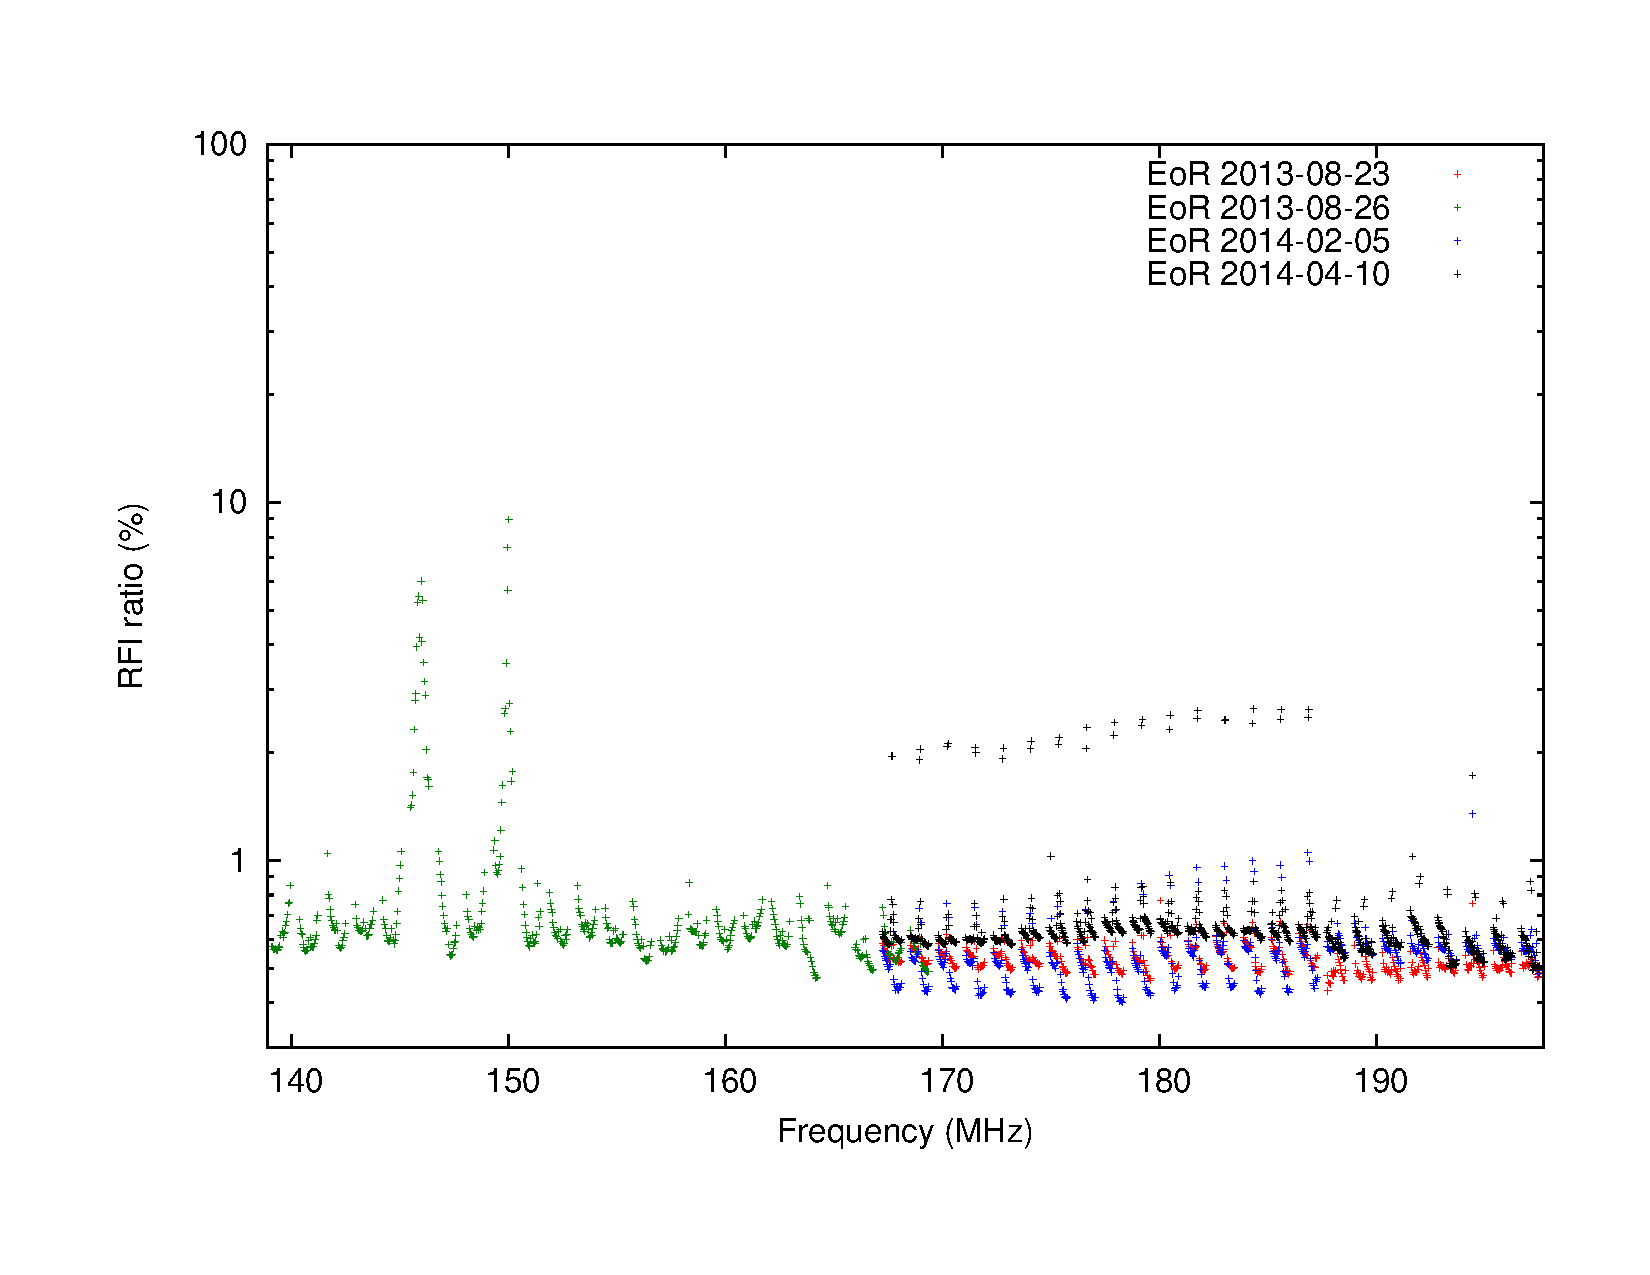
\includegraphics[width=18cm]{img/plot-rfi-per-set-eor}\vspace{-1cm}
%\caption{..}
%\label{fig:rfi-per-set-eor}
%\end{center}
%\end{figure*}

%\noindent\begin{figure*}
%\begin{center}\hspace*{-0.2cm}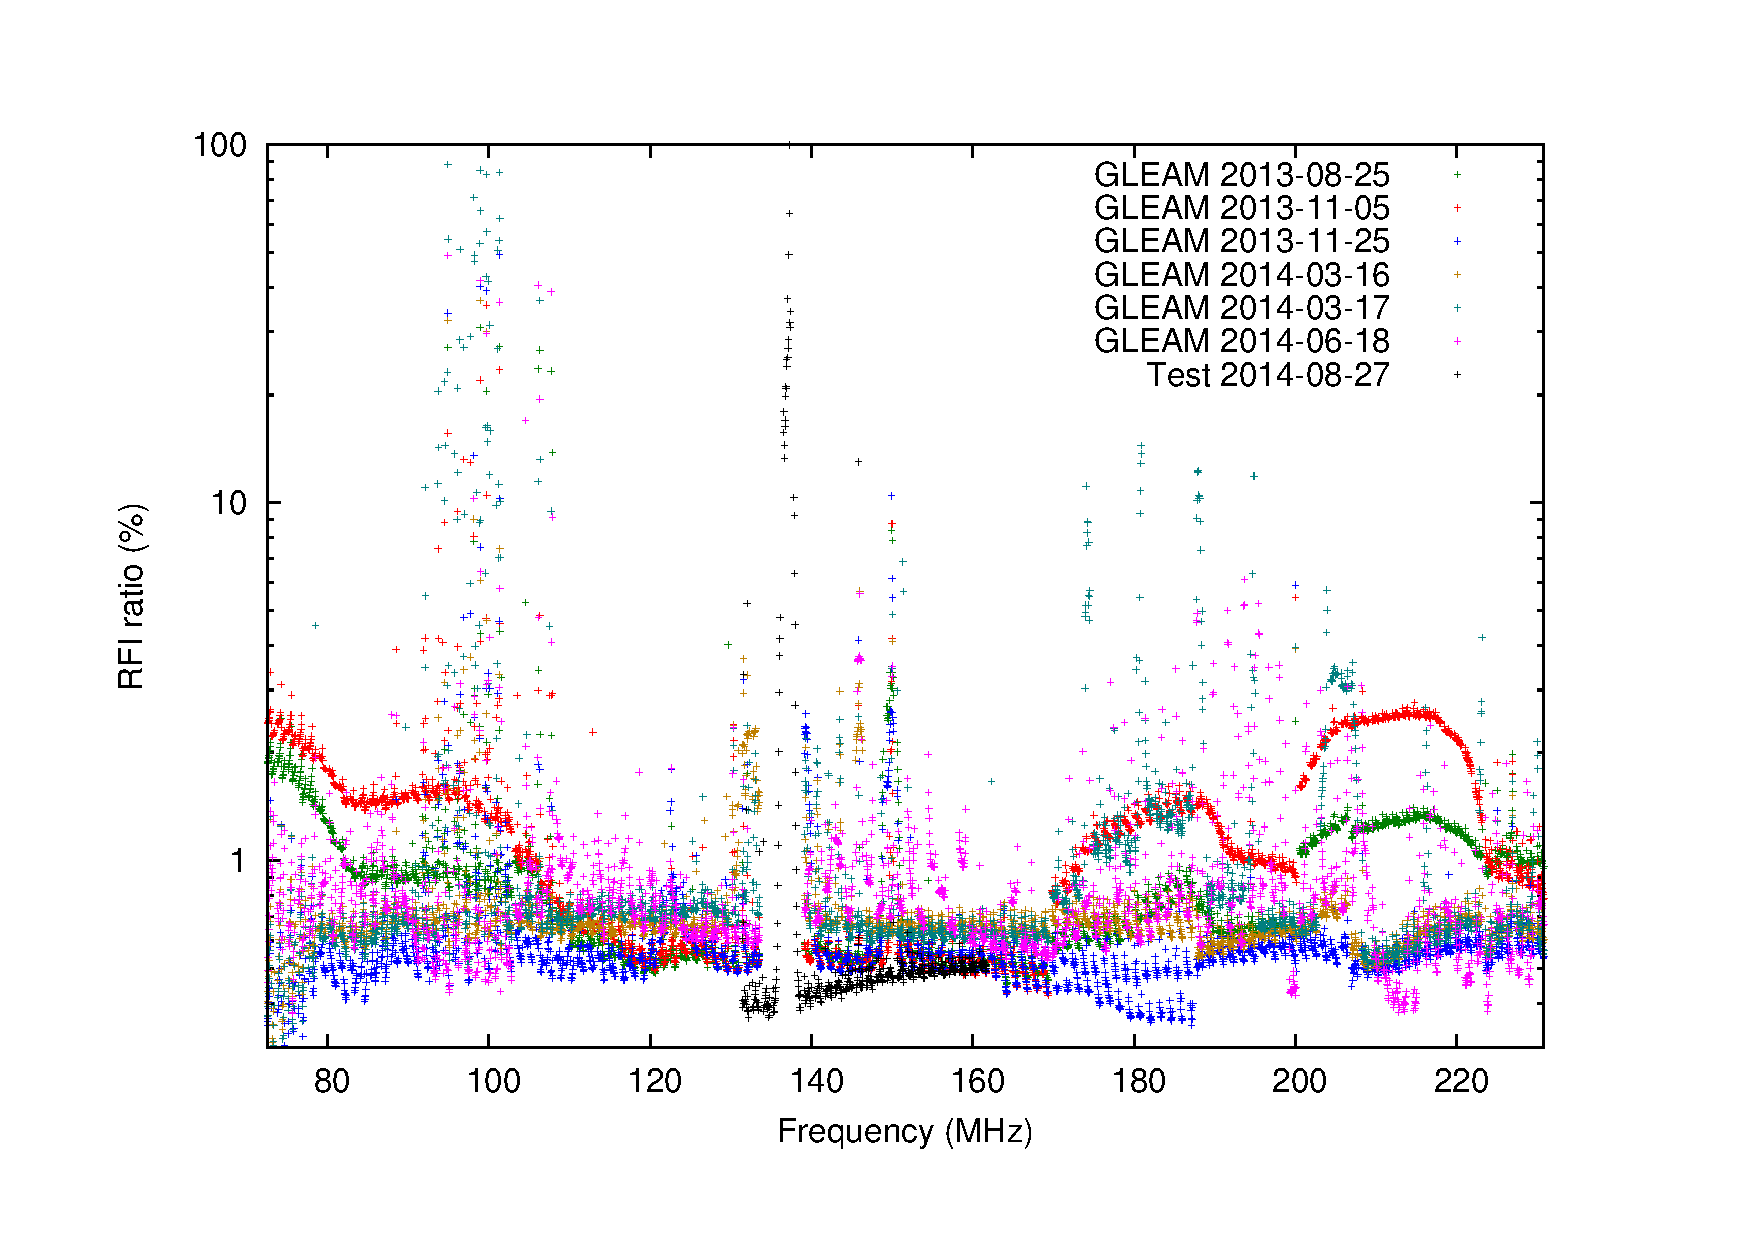
\includegraphics[width=18cm]{img/plot-rfi-per-set-gleam}\vspace{-1cm}
%\caption{..}
%\label{fig:rfi-per-set-gleam}
%\end{center}
%\end{figure*}

\noindent\begin{figure}
\begin{center}\hspace*{-0.2cm}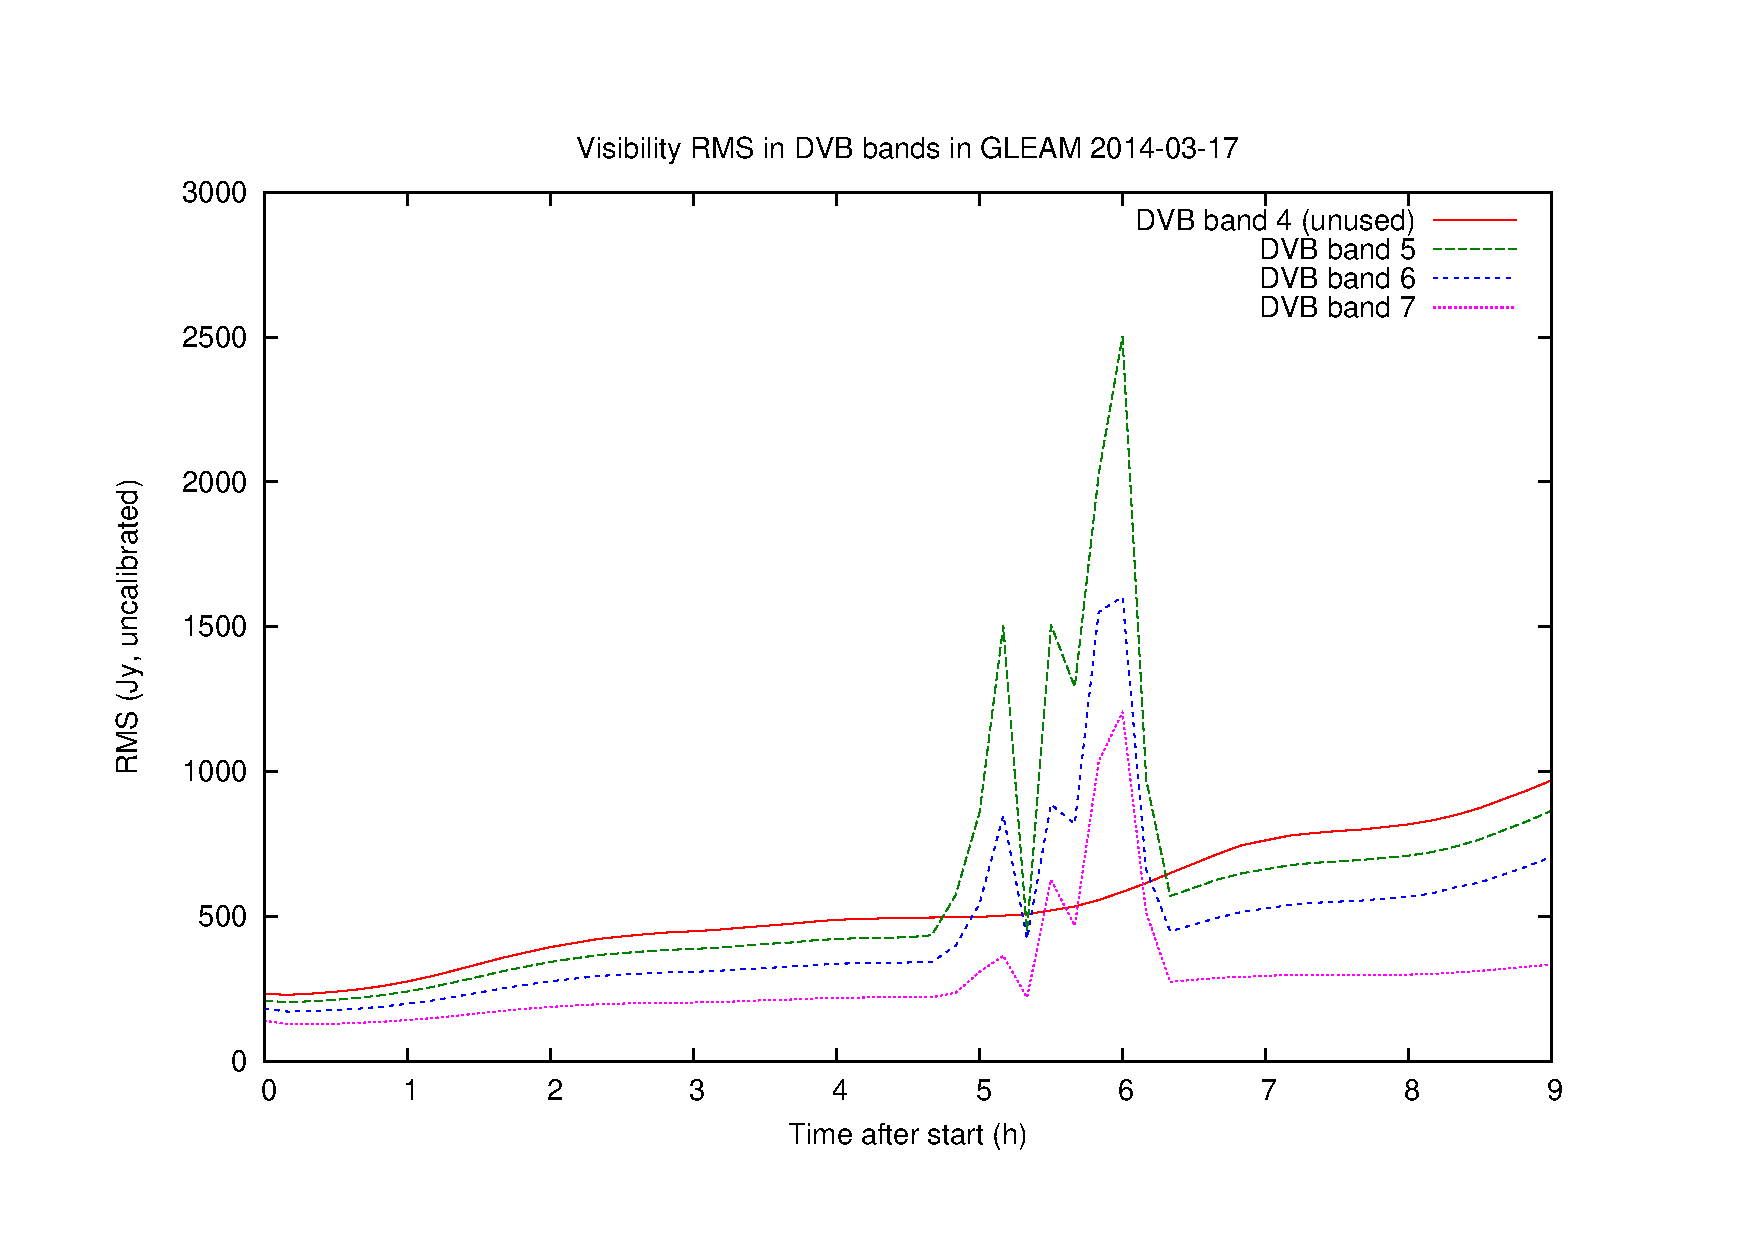
\includegraphics[width=9.1cm]{img/2014-03-17-dvb-stddevs}
\caption{..}
\label{fig:dvb-stddevs}
\end{center}
\end{figure}

\noindent\begin{figure*}
\begin{center}\hspace*{-0.2cm}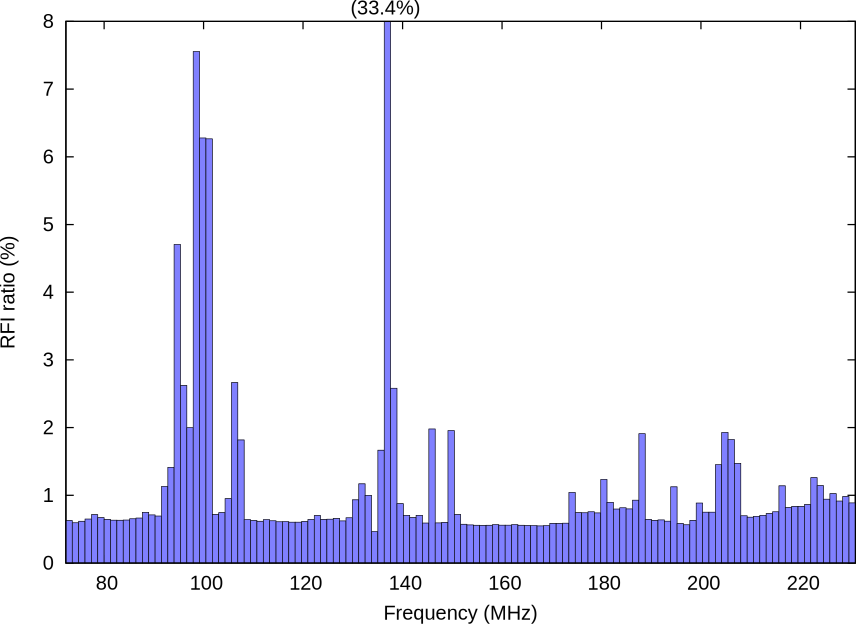
\includegraphics[width=18cm]{img/rfi-per-band}
\caption{RFI per subband}
\label{fig:rfi-per-band}
\end{center}
\end{figure*}

\noindent\begin{figure*}
\begin{center}\hspace*{-0.2cm}\includegraphics[width=18cm]{img/lognlogs-multiplot}
\caption{Log N log S}
\label{fig:lognlogs}
\end{center}
\end{figure*}

\begin{itemize}
 \item Total RFI statistics
 \item Percentages + stddev per frequency + discuss
 \item An example of RFI found (e.g., the EoR DVB, ..)
 \item Performance
 \item Log N log S Histograms
\end{itemize}

\section{Discussion}
\begin{itemize}
 \item SKA -- how to implement a Cotter for SKA?
\end{itemize}

\section{Conclusions}
\begin{itemize}
 \item Much less RFI than LOFAR (but at a cost)
 \item About half the observations don't need flagging at all. 
 \item FM not completely empty
\end{itemize}

\section*{Acknowledgments}
This scientific work makes use of the Murchison Radio-astronomy Observatory, operated by CSIRO. We acknowledge the Wajarri Yamatji people as the traditional owners of the Observatory site. Support for the MWA comes from the U.S. National Science Foundation (grants AST-0457585, PHY-0835713, CAREER-0847753, and AST-0908884), the Australian Research Council (LIEF grants LE0775621 and LE0882938), the U.S. Air Force Office of Scientific Research (grant FA9550-0510247), and the Centre for All-sky Astrophysics (an Australian Research Council Centre of Excellence funded by grant CE110001020). Support is also provided by the Smithsonian Astrophysical Observatory, the MIT School of Science, the Raman Research Institute, the Australian National University, and the Victoria University of Wellington (via grant MED-E1799 from the New Zealand Ministry of Economic Development and an IBM Shared University Research Grant). The Australian Federal government provides additional support via the Commonwealth Scientific and Industrial Research Organisation (CSIRO), National Collaborative Research Infrastructure Strategy, Education Investment Fund, and the Australia India Strategic Research Fund, and Astronomy Australia Limited, under contract to Curtin University. We acknowledge the iVEC Petabyte Data Store, the Initiative in Innovative Computing and the CUDA Center for Excellence sponsored by NVIDIA at Harvard University, and the International Centre for Radio Astronomy Research (ICRAR), a Joint Venture of Curtin University and The University of Western Australia, funded by the Western Australian State government. 

% To make Dutch ``tussenvoegsels'' work correctly in Latex such as ``de Bruyn'', we use this command
% In bibliography, it should be written with lowercase, as in ``de Bruyn''
\DeclareRobustCommand{\TUSSEN}[3]{#3}

\bibliographystyle{mn2e}
\bibliography{references}

\label{lastpage}

\end{document}
